\part{Theoretical foundations}

\chapter{Point Processes}
\label{chap-point_proc}

\section{Marked Spatio-Temporal Point Processes}
\label{sec-mark_point}

A spatio-temporal point process $\mathcal{X}$ is a sequence of random variables on $\{S \subset \mathds{R}^{2} \times [0,T]\}$ in which the number of points in $S \times T$ has a counting measure $N(S \times T)$ who is almost surely finite, when $S \times T$ is bounded. Usually $\mathcal{X}$ is observed in a spatio-temporal window $W = S \times T$, and a realization of $\mathcal{X}$ in $W$ is a set $\mathbf{x} = \{(s_{i},t_{i}), i = 1,2,\ldots,n\}$, where $s_{i} = (x_{i},y_{i})$ and $t_{i}$ represent the spatial coordinates and times of occurrence of the i-th event, respectively.

A marked spatio-temporal point process incorporates a uniquely associated component $m_{i}$ with each event of $\mathcal{X}$. In earthquake's catalogs, the marks $m_{i}$ usually denote the magnitude of each event, while $(s_{i},t_{i})$ represents the longitude/latitude of the earthquake's epicenter and the ordered times of occurrence.

\begin{table}[htb]
\IBGEtab{%
  \caption{Example of a earthquake catalog.}%
  \label{tab-catalog-example}
}{%
\begin{tabular}{ccccc}
  \toprule
   \textbf{Event} & \textbf{Time}  & \textbf{Longitude}  & \textbf{Latitude} & \textbf{Magnitude}  \\
  \hline
  1 & $t_{1}$ & $x_{1}$ & $y_{1}$ & $m_{1}$ \\
  2 & $t_{2}$ & $x_{2}$ & $y_{2}$ & $m_{2}$ \\
  \vdots & \vdots & \vdots & \vdots & \vdots \\
  n & $t_{n}$ & $x_{n}$ & $y_{n}$ & $m_{n}$ \\
  \bottomrule
\end{tabular}
}{%
  \fonte{The author.}
  }
\end{table}

Consider the event history $\mathcal{H}_{t} = \left\{(x_{i},y_{i},t_{i},m_{i}) \in \mathcal{X} : t_{i} < t\right\}$. A spatio-temporal point process can be fully characterized by it's conditional intensity function $\lambda(s,t | \mathcal{H}_{t})$ \cite{daley_jones_2003}
\begin{equation}
  \label{eq-intensity-function}
  \lambda(s,t|\mathcal{H}_{t}) = \lim_{\delta s,\delta t \to 0}\frac{\mathds{E}\left[N(\delta s \times \delta t)|\mathcal{H}_{t}\right]}{\delta s\, \delta t},
\end{equation}

\noindent that represents the expected number of events observed in an infinitesimal region of volume $(\delta s \times \delta t)$ centered around $(s, t)$, conditional in the observed history of the process up to time $t$. With it, we can define the process's associated compensator $\Lambda(t)$
\begin{equation}
  \label{eq-compensator}
  \Lambda(t|\mathcal{H}_{u}) = \int_{0}^{t}\int_{S}\lambda(s,u|\mathcal{H}_{u})ds\,du,
\end{equation}

\noindent in which $N(s,t|\mathcal{H}_{t}) - \Lambda(t|\mathcal{H}_{t})$ is an local $\mathcal{H}_{t}$-martingale. The simplest and most common kind of spatio-temporal point process is the Poisson Process, defined as such:

\begin{definition}[Poisson Process]
  \label{def-poisson-process}
  A spatio-temporal counting process $\{N(s,t): s \in \mathds{R}^{2},t \in \mathds{R}_{+}\}$ is a Inhomogeneous Poisson Process with intensity function $\lambda(s,t)$ if:
  \begin{itemize}
  \item For any bounded window $W = (S \times T)$, $N(W) \sim \mathrm{Pois}\left(\int_{T}\int_{S}\lambda(s,t)ds \, dt\right)$;
  \item For any $n$ disjoint windows $W_{1}, W_{2}, \ldots, W_{n}$, the random variables $N(W_{1}), N(W_{2}), \ldots, N(W_{n})$ are mutually independent.
  \end{itemize}
\end{definition}

The Poisson Process have two properties that makes it very versatile for modeling point processes in general: \textbf{Superposition} and \textbf{Thinning}:

\begin{theorem}[Superposition of Poisson Processes]
  \label{teo-superposition}
  Given $k$ independent Poisson Processes $\mathcal{X}_{1}, \mathcal{X}_{2}, \ldots, \mathcal{X}_{k}$ with intensity functions $\lambda_{1}, \lambda_{2}, \ldots, \lambda_{k}$, the new process $\mathcal{X} = \sum_{i=1}^{k}\mathcal{X}_{i}$ is a Poisson Process, with intensity function $\lambda = \sum_{i=1}^{k}\lambda_{i}$.
\end{theorem}

\begin{theorem}[Thinning of Poisson Processes]
  \label{teo-thinning}
  Let $\mathcal{X}$ be a Poisson Process with intensity function $\lambda$. For each occurrence of $\mathcal{X}$, assign it to process $\mathcal{X}_{1}$ with probability $p_{1}$, to process $\mathcal{X}_{2}$ with probability $p_{2}$, and so on up to process $\mathcal{X}_{k}$ with probability $p_{k}$, such that $\sum_{i=1}^{k}p_{i} = 1$. The new processes $\{\mathcal{X}_{1},\mathcal{X}_{2},\ldots, \mathcal{X}_{k}\}$ are Poisson Processes with intensity functions $\{p_{1}\lambda, p_{2}\lambda, \ldots, p_{k}\lambda\}$, and are mutually independent.
\end{theorem}

With these two results, many point processes can have their intensity function modelled using Poisson Processes. However, one condition necessary for that is that $\lambda(s,t)$ must remain constant along time (i.e. $\lambda(s,t) = \lambda(s),\, \forall t \in [0,T]$), and in many cases that is not necessarily true.

\section{Hawkes Processes and the ETAS Model}
\label{sec-hawkes_proc}

In many pontual phenomena, the ocurrence of events increases the probability of further events occuring, such as the spread of diseases, urban violence (\citeonline{mohler_2011}, \citeonline{ludwig_2025}) and earthquakes. For these kinds of processes, the intensity function must change dynamically, in order to accommodate the increase in probability triggered by a previous event.

A self-exciting point process (occuring in time) was proposed by \citeonline{hawkes_1971a}, having intensity function given by
\begin{equation}
  \label{eq-hawkes-uni}
  \lambda(t|\mathcal{H}_{t}) = \mu + \sum_{i:t_{i} < t}g(t - t_{i}),
\end{equation}

\noindent where $\mu > 0$ is the baseline intensity of the process, and $\sum_{i:t_{i} < t}g(t - t_{i})$ represents the contribution of past events to the increase in the conditional intensity up to time $t$, with $g(v) \ge 0$ for nonnegative $v$ and 0 otherwise. To guarantee stationarity for this process (\citeonline{hawkes_1971b}), is necessary that $\int_{0}^{\infty}g(v)dv < 1$, otherwise the process can have infinite events in finite time.

The \textbf{ETAS} (\textit{Epidemic-Type Aftershock Sequence}) Model was proposed by \citeonline{ogata_1988}, and is the most used to describe earthquake occurrences. The initial model was only concerned with the event times and was a particular case of a marked point process, for it's inclusion of the earthquake's magnitudes. This model assumes that any earthquake can come from one of two sources: the \textbf{background} events come from a Inhomogeneous Poisson Process, independent of time, and the \textbf{offspring} were triggered by a previous event (either a background, or another offspring). Another way to call these events are \textbf{aftershocks}, and have a more geological interpretation.  \autoref{fig-branching-process} shows the branching structure of a temporal \textbf{ETAS}, with events beign parents if they come from generation 0, and offsprings if they come from any other generation.

\begin{figure}[htb]
	\caption{\label{fig-branching-process}Branching of an self-exciting point process.}
	\begin{center}
	    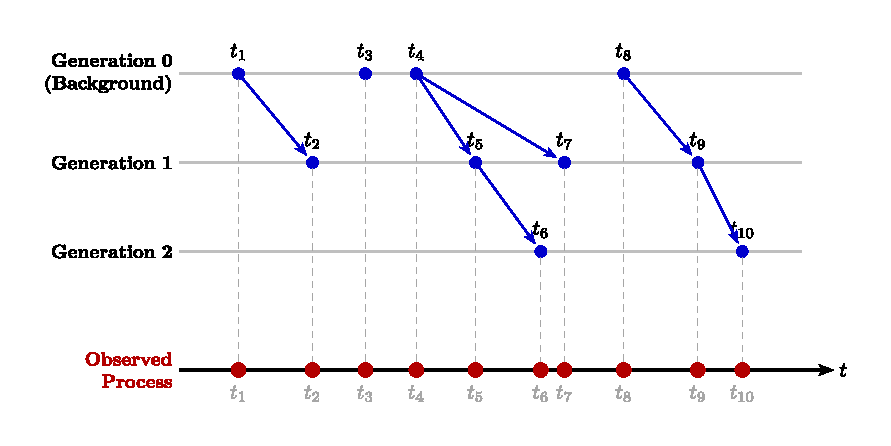
\includegraphics[scale=1]{Images/branching_process.pdf}
	\end{center}
\end{figure}

In a later work, \citeonline{ogata_1998} extended the ETAS model to accommodate the spatio-temporal distribution of earthquakes, in the form
\begin{equation}
  \label{eq-mod-etas}
  \lambda_{\theta}(x,y,t|\mathcal{H}_{t}) = \mu(x,y) + \sum_{i: t_{i} < t}\kappa(m_{i})g(t - t_{i};m_{i})f(x - x_{i}, y - y_{i};m_{i}),
\end{equation}

\noindent with it's components being:

\begin{itemize}
\item $\mu(x,y)$ is the background rate, representing a smooth function on the region $S$, with $\mu(x,y) > 0$. The parent events occur following this background rate, and it is assumed to be independent of time.
\item $\kappa(m_{i})$ is the productivity of the process, representing the expected number of events triggered from a event of magnitude $m_{i}$, taking form
  \begin{equation*}
    \kappa(m) = A\exp[\alpha(m - m_{0})],
  \end{equation*}
  with $A > 0$ and $\alpha > 0$ being unknown parameters, and $m_{0}$ the cutoff magnitude being considered in the study (i.e., all the $n$ events in the catalog have magnitudes $m_{i} \ge m_{0}, i = 1, 2,\ldots, n$).
\item $g(t - t_{i})$ is the probability density function of the time (in days) of a triggered event occuring at time $t_{i}$, and is assumed to be independent of the event magnitude $m_{i}$. A power law density is considered, based in the modified Omori's law (\citeonline{utsu_1995})
  \begin{equation*}
    g(t - t_{i}) =
    \begin{cases}
      (p - 1)c^{p-1}\left((t - t_{i}) + c\right)^{-p}, & t - t_{i} > 0 \\
      0, & t - t_{i} \le 0
    \end{cases},
  \end{equation*}
  with $c > 0$ and $p > 1$ being unknown parameters.
\item $f(x - x_{i}, y - y_{i};m_{i})$ is the probability density function of the location in space of a event triggered from a event occurred in $(x_{i}, y_{i})$ and magnitude $m_{i}$. The distances are considered to be in $\text{degrees}^{2}$ ($x$ is the longitude and $y$ is the latitude), and this can cause some considerable distortion in areas with big latitudes. An isotropic density function is considered
  \begin{equation*}
    f(x - x_{i}, y - y_{i};m_{i}) = \frac{q - 1}{\pi D \exp[\gamma(m_{i} - m_{0})]}\left(1 + \frac{(x - x_{i})^{2} + (y - y_{i})^{2}}{D \exp[\gamma(m_{i} - m_{0})]}\right)^{-q},
  \end{equation*}
  with $D > 0, \gamma > 0$ and $q > 1$ are unknown parameters.
\end{itemize}

Other parametrizations for $\lambda_{\theta}(x,y,t|\mathcal{H}_{t})$ were proposed by Ogata, but this one offers great flexibility by allowing the times of triggered events to be independent of the magnitudes, and by having separated parameters that control different aspects of the earthquake's intensity function behavior (temporal decay rate, influence of magnitudes in the number of expected offspring, spatial clustering, etc). The model can also incorporate the distribution of the marks/magnitudes
\begin{equation}
  \label{eq-model-eta-marks}
  \lambda_{\theta,\beta}(x,y,t,m|\mathcal{H}_{t}) = \nu(m)\lambda_{\theta}(x,y,t|\mathcal{H}_{t}),
\end{equation}

\noindent where $\nu(m)$ follows the Gutenberg-Richter distribution (\citeonline{gutenberg_1944})
\begin{equation*}
  \nu(m) = \beta\exp[-\beta(m - m_{0})], \,\, \beta > 0.
\end{equation*}

The expected number of offsprings generated from any event, regardless of its magnitude is given by
\begin{equation}
  \label{eq-expect-triggered}
  e_{\text{off}} = \int_{m_{0}}^{\infty}\kappa(m)\nu(m)dm = \frac{A\beta}{\beta - \alpha}.
\end{equation}

If $e_{\text{off}} < 1$, the model is stable (\citeonline{daley_jones_2003}), and has agglomerate size of $\frac{1}{(1 - e_{\text{off}})} = \frac{\beta - \alpha}{\beta(1 - A) - \alpha}$. Because the marks distribution is independent of the other parameters (as the complete intensity $\lambda_{\theta,\beta}(x,y,t,m|\mathcal{H}_{t})$ is the product of $\nu(v)$ and $\lambda_{\theta}(x,y,t|\mathcal{H}_{t})$), the estimation of $\beta$ can be done without the need to estimate the other parameters.

\section{Likelihood and Stochastic Declustering}
\label{sec-likelihood-etas}

Estimating the model parameters $\beta$ and $\theta = (A, \alpha, c, p, D, \gamma, q)$ and the background intensity function $\mu(x,y)$ is crucial to understand the seismological dynamic of a certain region, as it dictates when and where the aftershocks of an earthquake have more probability of happening. Moreover, early-warning systems depend on this estimates to make predictions in feasible time, as the time needed for these systems to mitigate further damages are between 1 and 10 minutes (\citeonline{allen_2019}).

For this, maximum likelihood methods for estimating the vector parameters have many desirable properties, such as being consistent, asymptotically unbiased and efficient (\citeonline{ogata_1978}). The ETAS model complete log-likelihood is given by
\begin{equation}
  \label{eq-etas-loglik}
  l(\theta,\beta|\mathcal{H}_{t}) = \sum_{i = 1}^{n}\log(\lambda_{\theta,\beta}(x_{i},y_{i},t_{i},m_{i}|\mathcal{H}_{t})) - \int_{m_{0}}^{\infty}\int_{0}^{T}\int\int_{S}\lambda_{\theta,\beta}(x,y,t,m|\mathcal{H}_{t})dx\, dy\, dt\, dm,
\end{equation}

\noindent where $T$ is the time of the last event in the catalog (the time integral starts at 0 because we can re-scale the event times $(t_{1},t_{2}, \ldots, t_{n})$ such that we have the fist event occur at time 0 with $(t_{1} - t_{1}, t_{2} - t_{1}, \ldots, t_{n} - t_{1}) = (0, t_{2}^{\ast}, \ldots, T)$). As seen in \autoref{eq-model-etas-marks}, $\beta$ and $\theta$ are separable, and $\int_{m_{0}}^{\infty}\nu(m)dm = 1$ (because it is a probability density function), we can decompose the previous log-likelihood as
\begin{equation*}
  l(\theta,\beta|\mathcal{H}_{t}) = l_{1}(\beta|\mathcal{H}_{t}) + l_{2}(\theta|\mathcal{H}_{t})
\end{equation*}

\noindent where
\begin{equation}
  \label{eq-loglik-beta}
  l_{1}(\beta|\mathcal{H}_{t}) = \sum_{i=1}^{n}\log(\nu(m_{i})) = n\log(\beta) - \beta\sum_{i=1}^{n}(m_{i} - m_{0})
\end{equation}

\noindent and
\begin{equation}
  \label{eq-loglik-theta}
  l_{2}(\theta|\mathcal{H}_{t}) = \sum_{i=1}^{n}\log(\lambda_{\theta}(x_{i},y_{i},t_{i}|\mathcal{H}_{t})) - \int_{0}^{T}\int\int_{S}\lambda_{\theta}(x,y,t|\mathcal{H}_{t})dx\, dy\, dt.
\end{equation}

The maximum likelihood estimator of $\beta$ can be obtained analytically using Equation \eqref{eq-loglik-beta}
\begin{equation*}
  \hat{\beta} = \frac{n}{\sum_{i=1}^{n}(m_{i} - m_{0})},
\end{equation*}

\noindent whereas the maximization of Equation \eqref{eq-loglik-theta} requires some form of numerical optimization method, to approximate the integral part. When we evaluate the integral term, we have
\begin{equation*}
  \int_{0}^{T}\int\int_{S}\lambda_{\theta}(x,y,t|\mathcal{H}_{t}) = T\int\int_{S}\mu(x,y) dx\, dy \, + \sum_{i:t_{i} < t}\kappa(m_{i})G(T - t_{i})F(S - s_{i};m_{i})
\end{equation*}

\noindent where $G(t)$ and $F(s)$ are the cumulative probability functions of $g(t)$ and $f(s)$, respectively, and are defined in \autoref{append-acum}. For any event not occurring near the spatio-temporal border (so that all the probability of being a offspring comes from the events inside the observed window, and not from any external event), we have that $G(T - t_{i}) \approx 1$ and $F(S - s_{i}) \approx 1$. This approximation simplifies the integral, making the log-likelihood easier to evaluate, when the assumptions are met.

However, the direct optimization of the complete log-likelihood remains complicated, due to two main factors: the $\log(\lambda_{\theta}(x_{i},y_{i},t_{i}|\mathcal{H}_{t}))$ term is the logarithm of a sum that has all the parameters and is not separable, and the computational cost for each evaluation is in the order of $\mathcal{O}(n^{2})$. If the underlying branching structure were known, the log-likelihood would be separable because the terms for the contribution of the background events and the offsprings would be either 1 or 0 for any occurrence.

Consider that each event $j$ has a parent $u_{j} \in \{0,1,\ldots,j-1\}$, in which $u_{j} = 0$ indicates a event that has come from the background rate function. If $u_{j}$ were observed, we would have
\begin{align}
  \begin{split}
  \label{eq-sep-loglik}
    l_{2}(\theta|\mathcal{H}_{t}) = &\sum_{j = 1}^{n}\left[\mathds{1}(u_{j} = 0)\log(\mu(x_{j},y_{j})) + \sum_{i < j}\mathds{1}(u_{j} \neq 0)\log(\kappa(m_{i})g(t_{j}-t_{i})f(s_{j} - s_{i};m_{i}))\right] - \\
                                    &T\int\int_{S}\mu(x,y)dx\, dy + \sum_{i:t_{i} < t}\kappa(m_{i})G(T - t_{i})F(S - s_{i};m_{i}),
\end{split}
\end{align}

\noindent making the log-likelihood separable, and with direct evaluation of the parameters. \citeonline{zhuang_2002} proposed a stochastic declustering method based on the decomposition of the conditional intensity in the ratio between the total intensity and the local intensity. Denote $\rho_{j}$ as the probability that the event $j$ is an background event, and $\rho_{ij}$ the probability that event $j$ was triggered by event $i$. Then, we have
\begin{equation}
  \label{eq-rho-j}
  \rho_{ij} = \frac{\kappa(m_{i})g(t_{j} - t_{i})f(s_{j} - s_{i};m_{i})}{\lambda_{\theta}(x_{j},y_{j},t_{j}|\mathcal{H}_{t_{j}})},
\end{equation}

\noindent and
\begin{equation}
  \label{eq-rho-ij}
  \rho_{j} = \frac{\mu(x_{j},y_{j})}{\lambda_{\theta}(x_{j},y_{j},t_{j}|\mathcal{H}_{t_{j}})} = 1 - \sum_{i<j}\rho_{ij}.
\end{equation}

Thus, the correct estimation of $\theta$ should in turn help estimate wheter an earthquake was triggerred by the background rate, or if it is an aftershock of another previous event in the catalog. When all the events in the catalog are far from the spatio-temporal border of the observed window $W$, we can consider the approximation $G(T - t_{i}) = F(S - s_{i};m_{i}) \approx 1$, and with the results from Equations \eqref{eq-rho-j} and \eqref{eq-rho-ij}, we can substitute the indicator function for the unobserved $u_{j}$'s in Equation \eqref{eq-sep-loglik} for their estimated probabilities as such
\begin{align}
  \begin{split}
    \label{eq-loglik-simp}
    l_{2}(\theta|\mathcal{H}_{t}) = &\sum_{j = 1}^{n}\rho_{j}\log\Big(\mu(x_{j},y_{j})\Big) + \sum_{i=1}^{n}\sum_{i < j}(1 - \rho_{j})\log\Big(\kappa(m_{i})g(t_{j} - t_{i})f(s_{j} - s_{i};m_{i})\Big) - \\
                                    &T\int\int_{S}\mu(x,y)dx\, dy + \sum_{i:t_{i} < t}\kappa(m_{i}).
  \end{split}
\end{align}

This form for the log-likelihood is easier to maximize given it's additive terms, but requires the calculated probabilities $\rho_{ij}$. The computational cost remains $\mathcal{O}(n^{2})$,

\part{Materials and Methods}

\chapter{Methods}
\label{chap-methods}

\section{Parameter Estimation}
\label{sec-parameter-estimation}

\section{Goodness of fit tests}
\label{sec-goodness_test}

\begin{theorem}[Random time change]
  \label{teo-mudanca-tempo}
  Let $0 < t_{1} < t_{2} < \ldots < t_{n}$ be the realization of a Point Process with conditional intensity function $\lambda(t|\mathcal{H}_{t})$, where $\lambda(t|\mathcal{H}_{t}) > 0$ for all $t \in [0,T]$. Then, the transformed times:
  \begin{equation*}
    \{\Lambda(t_{1}), \Lambda(t_{2}), \ldots, \Lambda(t_{n})\} = \{\tau_{1},\tau_{2},\ldots,\tau_{n}\},
  \end{equation*}
  are the points of a unidimensional unit rate Poisson Process, if $\Lambda(t|\mathcal{H}_{t})$ is almost surely finite for all $t \in [0,T]$.
\end{theorem}

This theorem holds for spatio-temporal point processes, and it is used for goodness of fit tests.
